\documentclass[a4paper, 12pt]{article}

\usepackage{makecell}
\usepackage{enumerate}
\usepackage{graphicx}
\usepackage[T5]{fontenc}
\usepackage[utf8]{inputenc}
\usepackage[margin = 2cm]{geometry}
\usepackage{amsfonts, amsmath, amssymb}
\usepackage[none]{hyphenat}
\usepackage{fancyhdr}
\usepackage{float}
\usepackage{hyperref}
\usepackage{caption}
\usepackage[nottoc, notlot, notlof]{tocbibind}
\usepackage{rotating}
\usepackage{tikz}

\captionsetup[table]{skip=5pt}
\pagestyle{fancy}
\fancyhead[L]{Trường Đại học Khoa học Tự nhiên - ĐHQG TP.HCM}
\fancyhead[R]{Nhóm Just $4^{th}$}

\begin{document}
    \begin{titlepage}
        \begin{center}
            % \begin{table}[htbp]
            %     \begin{center}
            %     \begin{tabular}{cc}
            %         \includegraphics[scale = 1]{images/Picture1.png} & \begin{tabular}[c]{@{}l@{}}Đại học Quốc gia TP.HCM\\ Trường Đại học Khoa học Tự nhiên\end{tabular}
            %     \end{tabular}
            %     \end{center}
            % \end{table}

            \vspace*{1cm}
            \Large\textbf{Báo cáo \#1\\Tài liệu yêu cầu phần mềm}\\

            \vfill
            \line(1,0){450}\\[4mm]
            \LARGE\textbf{\MakeUppercase{Dự án quản lý tạp chiếu phim}}\\[3mm]
            \Large{Nhập môn Công nghệ phần mềm (CSC13002)}\\[3mm]
            \Large{Nhóm Just $4^{th}$}
            \line(1,0){430}\\
            \vfill

            \vfill
            TP Hồ Chí Minh, ngày 20/10/2020
        \end{center}
    \end{titlepage}

    \tableofcontents
    \thispagestyle{empty}
    \clearpage

    \section{Thông tin nhóm}
    \label{sec:info}
    \begin{enumerate}
        \item \textbf{Đường link GitHub}: \url{https://github.com/baolongnguyenmac/CinemaManagementSystem}
        \item \textbf{Đường link Trello}: \url{https://trello.com/b/C0B4yLHF/báo-cáo-yêu-cầu}
        \item \textbf{Danh sách thành viên}
        \begin{table}[H]
            \begin{tabular}{|c|c|l|c|c|}
            \hline
            STT & MSSV     & \multicolumn{1}{c|}{Họ tên} & Email                         & SĐT        \\ \hline
            1   & 18120201 & Nguyễn Bảo Long             & 18120201@student.hcmus.edu.vn & 0919070940 \\ \hline
            2   & 18120211 & Võ Thế Minh                 & 18120211@student.hcmus.edu.vn & 0981850699 \\ \hline
            3   & 18120227 & Phạm Văn Minh Phương        & 18120227@student.hcmus.edu.vn & 0343049359 \\ \hline
            4   & 18120210 & Phạm Tống Bình Minh         & 18120210@student.hcmus.edu.vn & 0971877781 \\ \hline
            5   & 18120264 & Nguyễn Duy Vũ               & 18120264@student.hcmus.edu.vn & 0911572108 \\ \hline
            \end{tabular}
            \caption{Bảng danh sách thành viên nhóm}
        \end{table}
    \end{enumerate}
    \clearpage

    \section{Lịch sử cập nhật}
    \label{sec:history}
    \begin{table}[h]
        \begin{tabular}{|c|c|c|l|l|}
        \hline
        STT &Ngày cập nhật &Phiên bản &\multicolumn{1}{c|}{Mô tả chi tiết} &\multicolumn{1}{c|}{Tác giả} \\ \hline
        1 &22/10/2020 &1.0 &\begin{tabular}[c]{@{}l@{}}- Nhận diện thành viên nhóm\\ - Mô tả bài toán\\ - Yêu cầu hệ thống\\ - Xác định stakeholder\\ - Xác định actor\end{tabular} &\begin{tabular}[c]{@{}l@{}}Phạm Tống Bình Minh\\ Nguyễn Bảo Long\\ Nguyễn Duy Vũ\end{tabular} \\ \hline
        2 &25/10/2020 &1.1 &\begin{tabular}[c]{@{}l@{}}- Đặc tả use case\\ - Vẽ biểu đồ use case\\- Vẽ biểu đồ tuần tự\\ - Lên kế hoạch làm việc\end{tabular} &\begin{tabular}[c]{@{}l@{}}Phạm Tống Bình Minh\\ Nguyễn Duy Vũ\\Nguyễn Bảo Long \\ Võ Thế Minh\end{tabular} \\ \hline
        % 3 &25/10/2020 &1.2 &\begin{tabular}[c]{@{}l@{}}- Vẽ biểu đồ tuần tự\\ - Lên kế hoạch làm việc\end{tabular} &\begin{tabular}[c]{@{}l@{}}Nguyễn Bảo Long \\ Võ Thế Minh\end{tabular} \\ \hline
        % 4 &26/10/2020 &1.3 &- Đặc tả giao diện người dùng &Phạm Văn Minh Phương \\ \hline
        % 5 &26/10/2020 &1.5 &- Phân tích đóng góp cá nhân &Phạm Văn Minh Phương \\ \hline
        \end{tabular}
        \caption{Bảng lịch sử cập nhật các phiên bản của báo cáo yêu cầu}
    \end{table}
    \clearpage

    \section{Nhận diện thành viên}
    \label{sec:regconize}
    \begin{enumerate}
        \item Nguyễn Bảo Long - Nhóm trưởng
        \begin{itemize}
            \item Ưu điểm: Là người hướng tác vụ, có khả năng lên kế hoạch và xúc tiến quá trình làm việc của các thành viên khác, có tính cầu tiến
            \item Kỹ năng: Lập trình, trình bày, viết tài liệu, tổ chức kế hoạch
        \end{itemize}

        \item Võ Thê Minh
        \begin{itemize}
            \item Ưu điểm: Là người hướng tương tác, luôn quan tâm đến các thành viên trong nhóm, có khả năng duy trì thái độ hoà nhã vui vẻ trong nhóm
            \item Kỹ năng: Lập trình, tìm hiểu công cụ, tìm hiểu quy trình làm việc
        \end{itemize}

        \item Phạm Văn Minh Phương
        \begin{itemize}
            \item Ưu điểm: Là người hướng tương tác, có khả năng tiếng Anh và có mắt thầm mỹ tốt, khả năng phân tích yêu cầu, có tinh thần học hỏi
            \item Kỹ năng: Thiết kế đồ hoạ, làm bài trình chiếu
        \end{itemize}

        \item Phạm Tống Bình Minh
        \begin{itemize}
            \item Ưu điểm: Là người hướng tương tác và hướng tác vụ, luôn nghiêm túc trong lúc làm việc nhưng có thể tạo không khí thoải mái cho các thành viên khác
            \item Kỹ năng: Lập trình, tìm kiếm tài liệu tham khảo
        \end{itemize}

        \item Nguyễn Duy Vũ
        \begin{itemize}
            \item Ưu điểm: Là người hướng hướng tác vụ, có khả năng trình bày tốt, có tinh thần học hỏi cao, kỹ tính trong lúc làm việc, logic trong tư duy lập trình
            \item Kỹ năng: Lập trình OOP, thiết kế và lập trình cơ sở dữ liệu
        \end{itemize}
    \end{enumerate}
    \clearpage

    \section{Phân tích đóng góp cá nhân}
    \label{sec:analys}
    \clearpage

    \section{Mô tả bài toán}
    \label{sec:decribeProblem}

    \subsection{Tên dự án: Dự án Quản lý rạp chiếu phim}

    % \begin{itemize}
    %     \item Ngữ cảnh: Xuất phát từ việc người mua vé xem phim phải xếp hàng trong rạp chiếu; Sự phổ biến của công nghệ nói chung và công nghệ web nói riêng. Do đó, mọi người đều có thể tiếp cận các trang web một cách dễ dàng
    %     \item Mục tiêu: Tự động hoá quá trình bán vé của rạp chiếu; Đơn giản và giám chi phí hoá các khâu liên quan đến quản lý nhân lực và nội dung của rạp chiếu (lên lịch chiếu, quản lý nhân viên bán vé, ...)
    %     \item 
    %     \item phần phạm vi thiếu nhẹ con link, viết thành 1 đoạn văn ít nhất nửa trang a4
    %     \item 
    %     \item Phạm vi: Nhóm phát triển đi vào giải quyết vấn đề và mong muốn đạt được mục tiêu như trên trong phạm vi các hoạt động thường nhật của rạp chiếu phim (sẽ được định nghĩa chi tiết trong phần chức năng)
    %     \item Những chức năng/tác vụ nằng ngoài phạm vi nêu trên đều không được đề cập hay cài đặt trong phần mềm
    % \end{itemize}

    \subsection{Mô tả dự án}
    Đặt trong bối cảnh sự phát triển không ngừng của công nghệ, sự cập nhật liên tục của thông tin, việc tiếp cận thông tin nhanh và dễ dàng là hết sức cần thiết. Tính tất yếu của bối cảnh trên là sự phổ biết về các thiết bị thông minh, giúp cập nhật thông tin liên tục cho người sử dụng. 
    \\[3mm]
    Trong trường hợp cụ thể, xét mô hình rạp chiếu phim truyền thống, khách hàng muốn xem phim cần thực hiện những thủ tục hết sức phiền phức. Nhóm phát triển xin được phép liệt kê một vài thử tục cho tới nay đã bị coi là lỗi thời như sau:
    \begin{itemize}
        \item Người xem phải xếp hàng chờ mua vé
        \item Chi phí thuê nhân viên bán vé rất tốn kém trong khi số lượng vé bán ra tại một thời điểm lại rất thấp
        \item Chi phí quảng cáo(in poster, tờ rơi,...) rất cao nhưng không mang lại hiệu quả như mong muốn
        \item Các thống kê về doanh thu được thực hiện thủ công và bất đồng bộ\footnote{Dữ liệu khó tổ chức và sao lưu do được thực hiện rời rạc, thủ công và không áp dụng các công nghê lưu trữ như Google Drive, Cloud,...}
    \end{itemize}
    Nhận thấy được các bất cập trong quy trình cũng như giới hạn trong xử lý công việc một cách thủ công của con người, nhóm phát triển đề xuất mô hình \textbf{Quản lý rạp chiếu phim} trên nền tảng web với một cách tiếp cận mới trong việc giải quyết các bất cập trên như sau:
    \begin{itemize}
        \item Hệ thống website cho phép người xem đặt vé online giúp cho việc xếp hàng chờ đến lượt mua vé không còn là vấn đề phải quan tâm
        \item Hệ thống website cập nhật liên tục thông tin về phim và lịch chiếu để người xem có thể tiếp cận dễ dàng
        \item Hệ thống website cho phép đăng thông tin quảng cáo để giảm chi phí poster, tờ rơi,... nhưng hiệu quả tiếp cận người dùng lại cao hơn nhiều so với phươgn pháp truyền thống.
    \end{itemize}
    Các ý trong phần liệt kê bên trên là một phần trong những giải pháp mà hệ thống cung cấp, giúp cho việc quản lý, vận hành rạp chiếu phim đạt hiệu quả cao trong khi chi phí lại thấp hơn nhiều so với việc áp dụng phương pháp quản lý truyền thống.

    \subsection{Yêu cầu người dùng}
    Chức năng \textbf{Đăng nhập, Đăng xuất, Đăng ký tài khoản} dành cho đối tượng người dùng là \textit{khách hàng của rạp phim}. Đối với chức năng \textbf{Đăng nhập}, \textit{khách hàng của rạp phim} cung cấp thông tin đăng nhập cho hệ thống. Theo đó, hệ thống sẽ xác thực và cho phép họ truy cập vào hệ thống nếu thông tin đúng hoặc không cho phép truy cập hệ thống nếu thông tin sai.
    \textit{Khách hàng của rạp phim} thực hiện chức năng \textbf{Đăng xuất} để xác nhận thoát khỏi hệ thống. Chức năng \textbf{Đăng ký} cho phép \textit{khách hàng của rạp phim} tạo tài khoản để truy cập vào hệ thống.
    \\\\
    Nhằm mục đích giúp \textit{khách hàng của rạp phim} linh hoạt trong việc mua vé, hệ thống cần có chức năng \textbf{Đăt, Huỷ vé} dành cho đối tượng người dùng là \textit{khách hàng của rạp phim}. Hai chức năng này cho phép \textit{khách hàng của rạp phim}, sau khi đăng nhập, có thể đặt vé hoặc huỷ vé đã đặt. Đối với chức năng \textbf{Đặt vé}, sau khi đặt vé thành công, hệ thống sẽ lock\footnote{không cho phép khách hàng khác đặt vé tại vị trí chỗ ngồi này} vị trí này trong 5 phút. Lưu ý, khi \textit{khách hàng của rạp phim} huỷ vé đã được thanh toán, hệ thống sẽ không hoàn lại tiền.
    \\\\
    Nhằm mục đích giúp cho \textit{khách hàng của rạp phim} có thể tiếp cận nhanh chóng với thông tin phim, hệ thống cần có chức năng \textbf{Xem thông tin phim} dành cho đối tượng người dùng là \textit{khách hàng của rạp phim}. Khi sử dụng chức năng này, \textit{khách hàng của rạp phim} có thể xem thông tin về phim, lịch chiếu và các chương trình khuyến mãi của rạp phim.
    \\\\
    Nhằm mục đích tạo ra sự thuật tiện trong việc thanh toán, hệ thống cần có chức năng \textbf{Thanh toán online qua ví điện tử Momo} dành cho đối tượng người dùng là \textit{khách hàng của rạp phim}. Khi sử dụng chức năng này, \textit{khách hàng của rạp phim} có thể sử dụng ví điện tử Momo của mình để thanh toán trước vé đã đặt.
    \\\\
    Chức năng \textbf{Đăng nhập, Đăng xuất} dành cho đối tượng người dùng là \textit{quản lý của rạp phim}. Khi sử dụng chức năng này, các \textit{quản lý của rạp phim} thực hiện truy cập vào hệ thống thông bằng chức năng \textbf{Đăng nhập} (cùng cấp thông tin đăng nhập cho hệ thống) và thoát khỏi hệ thống thông qua chức năng \textbf{Đăng xuất}.
    \\\\
    Nhằm mục đích tin học hoá cho quá trình cập nhật thông tin về phim, hệ thống cần có chức năng \textbf{Quản lý thông tin phim} dành cho đối tượng người dùng là \textit{quản lý của rạp phim}. Khi sử dụng chức năng này, \textit{quản lý của rạp phim} có thể thực hiện các thao tác \textbf{thêm, xoá, sửa thông tin của các phim trong rạp phim} (bao gồm lịch chiếu, thông tin giới thiệu phim, trailer).
    \\\\
    Nhằm mục đích tin học hoá cho quá trình cập nhật các chương trình khuyến mãi, hệ thống cần có chức năng \textbf{Quản lý các chương trình khuyến mãi} dành cho tối tượng người dùng là \textit{quản lý của rạp phim}. Khi sử dụng chức năng này, \textit{quản lý của rạp phim} có thể thực hiện các thao tác \textbf{thêm, xoá, sửa các chương trình khuyến mãi} của rạp phim.
    \\\\
    Chức năng \textbf{Đăng nhập, Đăng xuất} dành cho đối tượng người dùng là \textit{admin}. Khi sử dụng chức năng này, \textit{admin} thực hiện truy cập vào hệ thống thông bằng chức năng \textbf{Đăng nhập} (cùng cấp thông tin đăng nhập cho hệ thống) và thoát khỏi hệ thống thông qua chức năng \textbf{Đăng xuất}.
    \\\\
    Nhằm mục đích tạo ra sự dễ dàng trong quá trình quản lý và truy xuất thông tin của các \textit{quản lý của rạp phim}, hệ thống cần có chức năng \textbf{Quản lý các quản lý} dành cho đối tượng người dùng là \textit{admin}. Khi sử dụng chức năng này, \textit{admin} có thể thực hiện các thao tác \textbf{thêm, xoá, sửa các quản lý} của rạp phim.
    \\\\
    Nhằm mục đích tự động hoá quá trình thống kê doanh thu và đồng bộ hoá dữ liệu doanh thu, hệ thống cần có chức năng \textbf{Thống kê doanh thu} dành cho đối tượng người dùng là \textit{admin}. Khi sử dụng chức năng này, \textit{admin} có thể thực hiện các thống kê doanh thu theo phim, ngày, tháng hoặc năm.
    \clearpage

    \section{Yêu cầu hệ thống}
    \label{sec:requirement}

    \subsection{Định nghĩa thanh trọng số}
    \begin{itemize}
        \item 1: Ưu tiên rất cao 
        \item 2: Ưu tiên cao 
        \item 3: Ưu tiên trung bình 
        \item 4: Ưu tiên thấp 
    \end{itemize}

    \subsection{Yêu cầu chức năng}
    \begin{itemize}
        \item \textbf{Định nghĩa ID}
        \begin{itemize}
            \item ID có dạng a.b
            \item a nhận các giá trị $1, 2, 3$. $a = 1$ ám chỉ những yêu cầu chức năng liên quan đến đối tượng người dùng là \textit{khách hàng của rạp phim}, $a = 2$ ám chỉ những yêu cầu chức năng liên quan đến đối tượng người dùng là \textit{quản lý của rạp phim}, $a = 3$ ám chỉ những yêu cầu liên quan đến đối tượng người dùng là \textit{admin}
            \item b là số thứ tự
        \end{itemize}

        \item \textbf{Chi tiết yêu cầu chức năng}
        \begin{table}[h]
            \begin{tabular}{|c|c|l|}
                % tách các chức năng ra thành từng dòng riêng 
            \hline
            ID  & Trọng số  & \multicolumn{1}{c|}{Yêu cầu chức năng}                                                                                                          \\ \hline
            1.1 &     2     & Hệ thống sẽ cho phép \textit{khách hàng của rạp phim} \textbf{Đăng ký} tài khoản của họ     \\ \hline
            1.2 &     2     & Hệ thống sẽ cho phép \textit{khách hàng của rạp phim} \textbf{Đăng nhập} tài khoản của họ     \\ \hline
            1.3 &     2     & Hệ thống sẽ cho phép \textit{khách hàng của rạp phim} \textbf{Đăng xuất} tài khoản của họ     \\ \hline
            1.4 &     1     & Hệ thống sẽ cho phép \textit{khách hàng của rạp phim} \textbf{Đặt vé xem phim} \\ \hline
            1.5 &     1     & \begin{tabular}[c]{@{}l@{}}Hệ thống sẽ cho phép \textit{khách hàng của rạp phim} \textbf{Huỷ vé xem phim} (chỉ huỷ\\ được trong TH đã đặt vé trước đó)\end{tabular} \\ \hline
            1.6 &     2     & \begin{tabular}[c]{@{}l@{}}Hệ thống sẽ cho phép \textit{khách hàng của rạp phim} \textbf{Xem thông tin phim}\\(lịch chiếu, chương trình khuyến mãi)\end{tabular} \\ \hline
            1.7 &     2     & \begin{tabular}[c]{@{}l@{}}Hệ thống sẽ cho phép \textit{khách hàng của rạp phim} \textbf{thanh toán} vé đã đặt online\\ \textbf{qua ví điện tử Momo}\end{tabular}  \\ \hline
            2.1 &     2     & \begin{tabular}[c]{@{}l@{}}Hệ thống sẽ cho phép \textit{quản lý của rạp phim} \textbf{Đăng nhập} tài khoản do \textit{admin} cấp\end{tabular}         \\ \hline
            2.2 &     2     & \begin{tabular}[c]{@{}l@{}}Hệ thống sẽ cho phép \textit{quản lý của rạp phim} \textbf{Đăng xuất} tài khoản do \textit{admin} cấp\end{tabular}         \\ \hline
            2.3 &     1     & Hệ thống sẽ cho phép \textit{quản lý của rạp phim} \textbf{Quản lý thông tin phim} trong rạp                                                         \\ \hline
            2.4 &     4     & \begin{tabular}[c]{@{}l@{}}Hệ thống sẽ cho phép \textit{quản lý của rạp phim} \textbf{Quản lý các chương trình}\\ \textbf{khuyến mãi} trong rạp\end{tabular}\\ \hline
            3.1 &     2     & Hệ thống sẽ cho phép \textit{admin} \textbf{Đăng nhập} tài khoản của họ                                                                        \\ \hline
            3.2 &     2     & Hệ thống sẽ cho phép \textit{admin} \textbf{Đăng xuất} tài khoản của họ                                                                        \\ \hline
            3.3 &     3     & Hệ thống sẽ cho phép \textit{admin} \textbf{Quản lý các quản lý} trong rạp                                                                                \\ \hline
            3.4 &     4     & \begin{tabular}[c]{@{}l@{}}Hệ thống sẽ cho phép \textit{admin} \textbf{Thực hiện các thống kê về doanh thu} theo\\phim, ngày, tháng, năm\end{tabular}    \\ \hline
            \end{tabular}
            \caption{Bảng yêu cầu chức năng của hệ thống}
        \end{table}
    \end{itemize}

    \subsection{Yêu cầu phi chức năng}
    \begin{table}[H]
        \begin{tabular}{ccl} \hline
            \multicolumn{1}{|c|}{ID} & \multicolumn{1}{c|}{Trọng số} & \multicolumn{1}{c|}{Yêu cầu phi chức năng} \\ \hline
            \multicolumn{1}{|c|}{1} & \multicolumn{1}{c|}{1} & \multicolumn{1}{l|}{\begin{tabular}[c]{@{}l@{}}Thời gian phát triển phần mềm gói   gọn trong 12 tuần (tính từ lúc viết báo cáo \\ yêu cầu đến lúc hoàn thiện phần mềm)\end{tabular}} \\ \hline
            \multicolumn{1}{|c|}{2} & \multicolumn{1}{c|}{1} & \multicolumn{1}{l|}{\begin{tabular}[c]{@{}l@{}}Hệ thống sẽ lưu thông tin về mật khẩu của người dùng trong database sau khi \\được mã hoá\end{tabular}} \\ \hline
            \multicolumn{1}{|c|}{3} & \multicolumn{1}{c|}{3} & \multicolumn{1}{l|}{\begin{tabular}[c]{@{}l@{}}Thời gian phản hồi của hệ thống dưới 1s trong mọi chức năng trong môi trường\\ lý tưởng (sẽ định nghĩa lại sau)\end{tabular}} \\ \hline
            \multicolumn{1}{|c|}{4} & \multicolumn{1}{c|}{2} & \multicolumn{1}{l|}{Quy trình áp dùng: phát triển dần dần + tái sử dụng}     \\ \hline
            \multicolumn{1}{|c|}{5} & \multicolumn{1}{c|}{1} & \multicolumn{1}{l|}{\begin{tabular}[c]{@{}l@{}}Giao diện đảm bảo người dùng sử dụng được các chức năng cơ bản (đặt vé,\\ thanh toán online, xem lịch chiếu) trong tối đa 10p làm quen.\end{tabular}} \\ \hline
                                &                               &                                                                             
        \end{tabular}
        \caption{Bảng yêu cầu phi chức năng của hệ thống}
    \end{table}
    \clearpage

    \section{Đặc tả yêu cầu chức năng}
    \label{sec:describeFunction}

    \subsection{Danh sách các stakeholder}
    \begin{itemize}
        \item Người sử dụng trang web: Thông tin của họ được lưu trong hệ thống
        \item Quản lý: Là người quản lý các thông tin về phim, lịch chiếu và các chương trình khuyến mãi
        \item Admin: Là người quản lý các quản lý và thực hiện các thống kê doanh thu 
        \item Nhà sản xuất phim: Chịu trách nhiệm về nội dung, thời gian ra mắt, gắn nhãn giới hạn độ tuổi cho phim
        \item Bộ Văn hoá Thông tin \& Tuyền thông: Chịu trách nhiệm kiểm duyệt nội dung phim
    \end{itemize}

    \subsection{Danh sách các actor}
    \begin{itemize}
        \item User: Người sử dụng dịch vụ trang web để đặt vé xem phim, thanh toán online, xem thông tin phim và lịch chiếu
        \item Quản lý: Chịu trách nhiệm quản lý thông tin phim, lịch chiếu và các chương trình khuyến mãi
        \item Admin: Chịu trách nhiệm quản lý các quản lý và thực hiện các báo cáo thống kê về doanh thu 
    \end{itemize}

    \subsection{Đặc tả use case và vẽ biểu đồ use case}

    \subsubsection{Mô tả}
    \begin{table}[h]
        \begin{tabular}{|c|c|l|}
        \hline
        ID & Tên use case & \multicolumn{1}{c|}{Mô tả}                                                                         \\ \hline
        1   & Đăng nhập    & \begin{tabular}[c]{@{}l@{}}Giúp \textit{khách hàng của rạp phim, quản lý của rạp, admin} có thể đăng \\nhập vào tài khoản của mình trên hệ thống      \end{tabular}\\ \hline
        2   & Đăng ký      & Giúp \textit{khách hàng của rạp phim} tạo tài khoản cho bản thân trên hệ thống.                                      \\ \hline
        3   & Đăng xuất    & \begin{tabular}[c]{@{}l@{}}Giúp \textit{khách hàng của rạp phim, quản lý của rạp, admin} có thể thoát\\ khỏi tài khoản đang đăng nhập trên hệ thống \end{tabular}\\ \hline
        4   & Đặt vé       & Giúp \textit{khách hàng của rạp phim} có thể đặt vé xem phim trên hệ thống.                                          \\ \hline
        5   & Hủy vé       & \begin{tabular}[c]{@{}l@{}}Giúp \textit{khách hàng của rạp phim} có thể hủy vé xem phim đã đặt trước \\đó trên hệ thống                           \end{tabular}\\ \hline
        6   & \begin{tabular}[c]{@{}c@{}}Xem thông\\ tin phim\end{tabular}               & \begin{tabular}[c]{@{}l@{}}Giúp “Khách hàng” xem được thông tin các bộ phim đang được chiếu\\ trên hệ thống \end{tabular}\\ \hline
        7   & Thanh toán   & giúp “Khách hàng” thanh toán tiền mua vé trên hệ thống.                                          \\ \hline
        8   & \begin{tabular}[c]{@{}c@{}}Quản lý\\ lịch chiếu\end{tabular}               & Giúp \textit{quản lý của rạp} có thể chỉnh sửa lịch chiếu trên hệ thống.                     \\ \hline
        9   & \begin{tabular}[c]{@{}c@{}}Quản lý chương \\ trình khuyến mãi\end{tabular} & \begin{tabular}[c]{@{}l@{}}Giúp \textit{quản lý của rạp} có thể chỉnh sửa chương trình khuyến mãi trên\\ hệ thống      \end{tabular} \\ \hline
        10  & \begin{tabular}[c]{@{}c@{}}Quản lý tài khoản\\ các quản lý\end{tabular}    & Giúp \textit{admin} có thể chỉnh sửa các tài khoản quản lý trên hệ thống.            \\ \hline
        11  & \begin{tabular}[c]{@{}c@{}}Thống kê \\ doanh thu\end{tabular}              & Giúp \textit{admin} thống kê doanh thu của các rạp phim trên hệ thống                 \\ \hline
        \end{tabular}
    \end{table}

    \subsubsection{Biểu đồ use case}
    \begin{figure}[H]
        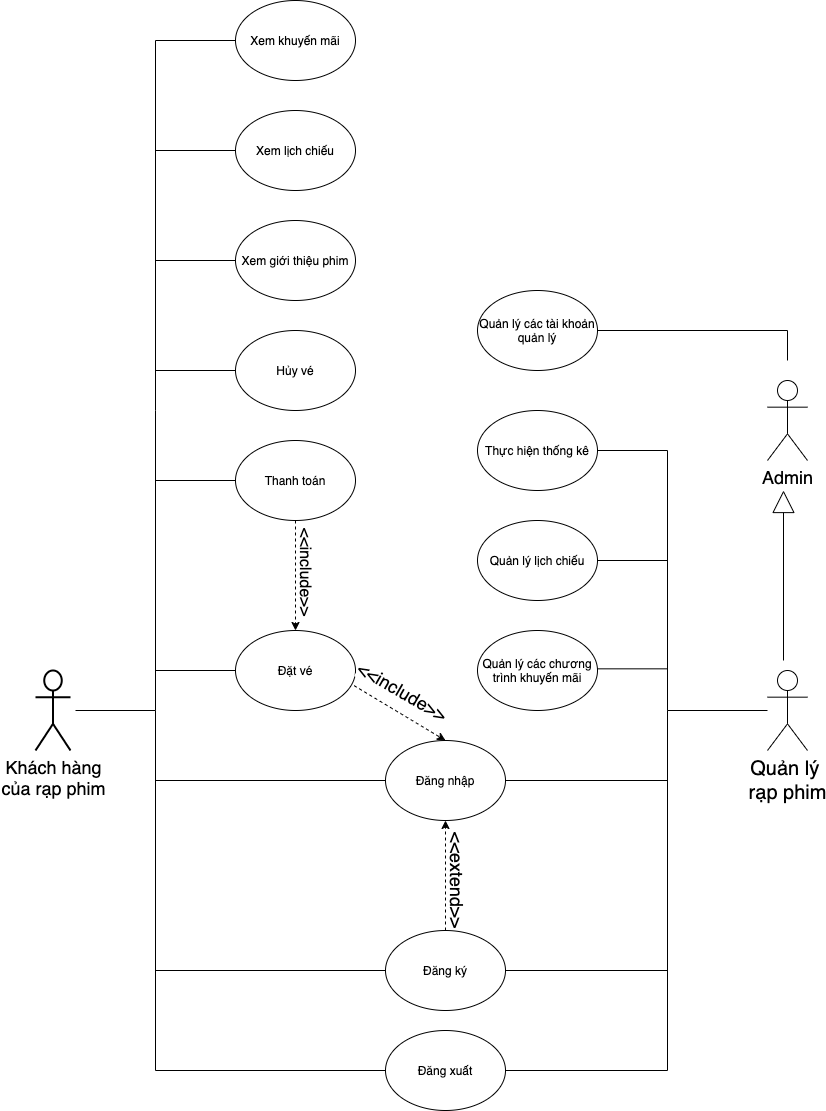
\includegraphics[scale = 0.5]{./UsecaseDiagram/usecase.png}
        \caption{Biểu đồ use case của hệ thống}
    \end{figure}

    \subsubsection{Ma trận truy xuất nguồn gốc}
    \begin{figure}[H]
        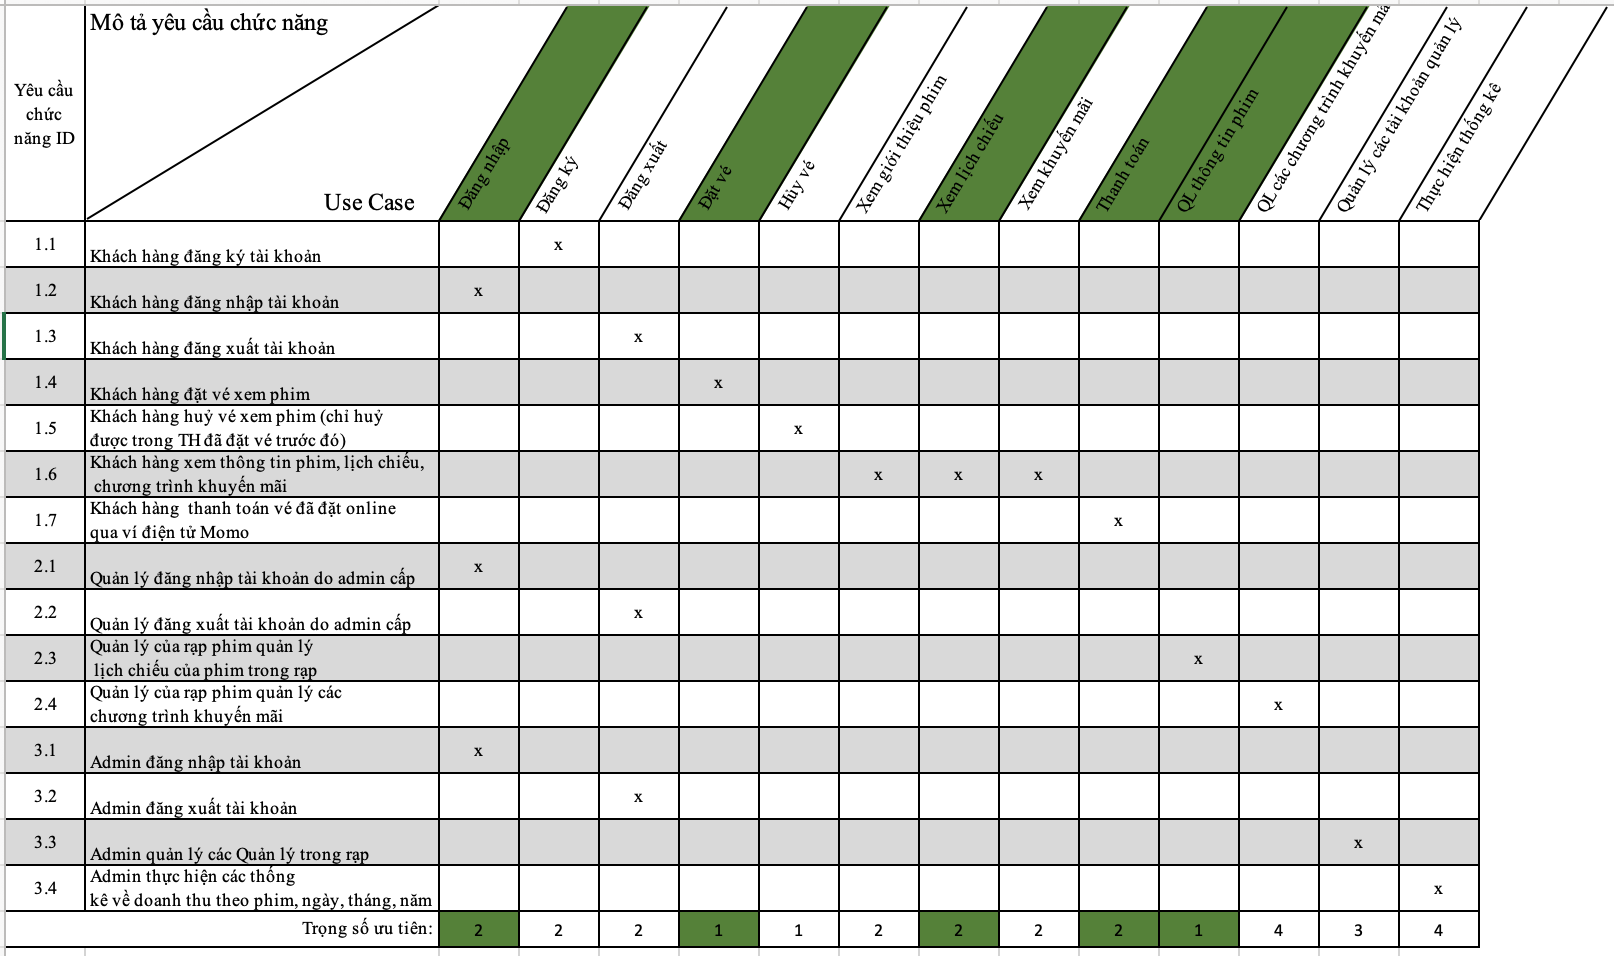
\includegraphics[scale = 0.7]{TraceMatrix/traceMatrix.png}
    \end{figure}

    \subsubsection{Đặc tả use case}


    \subsection{Biểu đồ tuần tự}
    \clearpage

    \section{Đặc tả giao diện người sử dụng}
    \label{sec:describeUI}
    \clearpage

    \section{Kế hoạch làm việc}
    \label{sec:plan}
    \clearpage

    \section{Tham khảo}
    \label{sec:reference}
    \clearpage

\end{document}